\documentclass[usenames,dvipsnames]{beamer}
\usepackage[noend]{algorithmic}
\usepackage{paralist}
\usepackage{latexsym,amsmath,url}
\usepackage{hyperref}
\usepackage{color}
\DeclareSymbolFont{AMSb}{U}{msb}{m}{n}
\DeclareMathSymbol{\N}{\mathbin}{AMSb}{"4E}
 \DeclareMathOperator*{\argmax}{argmax}

\newcommand{\vecb}[1]{\mathbf{#1}}
\newcommand{\x}{\mathbf{x}} 
\newcommand{\y}{\mathbf{y}}
\newcommand{\z}{\mathbf{z}}

\newcommand{\w}{\mathbf{w}}
\newcommand{\voc}[1]{{\color{ForestGreen}#1}}
\newcommand{\superscript}[1]{\ensuremath{^\textrm{\scriptsize#1 }}}
\mode<presentation>{ 
  \usetheme{Boadilla}
  %\setbeamercovered{invisible}
  % or whatever (possibly just delete it)
} \title[Sequences]{Sequence Labeling}


\author[Stroppa and Chrupala]{Grzegorz Chrupa{\l}a and Nicolas Stroppa}

\institute[UdS] % (optional, but mostly needed)
{
Google\\
Saarland University
}
\date[2010] % (optional, should be abbreviation of conference name)
{META}


\pgfdeclareimage[height=1cm]{UdS}{SaarlandUniversityLogo.jpg}
%\logo{\pgfuseimage{UdS}}

 \AtBeginSection[]
 {
    \begin{frame}
        \frametitle{Outline}
        \tableofcontents[currentsection]
    \end{frame}
 }
\begin{document}
\frame{\titlepage}

\begin{frame}
  \frametitle{Outline}
  \tableofcontents
\end{frame}

\begin{frame}
  \frametitle{Entity recognition in news}
  \begin{block}
    {}
West Indian all-rounder \alert{Phil Simons}$_{\text{PERSON}}$ took four for 38 on Friday as
Leicestershire ... 
  \end{block}
  \begin{itemize}
  \item We want to categorize news articles based on which entities
    they talk about
  \item We can annotate a number of articles with appropriate labels
  \item And learn a model from the annotated data
  \item Assigning labels to words in a sentence is an example of a
    \voc{sequence labeling} task
  \end{itemize}
\end{frame}

\begin{frame}
  \frametitle{Sequence labeling}
  \begin{center}
    \begin{small}
  \begin{tabular}{lll|l}
    Word        & POS    & Chunk     & NE      \\\hline
    West        & NNP    & B-NP      & B-MISC  \\
    Indian      & NNP    & I-NP      & I-MISC  \\
    all-rounder & NN     & I-NP      & O       \\
    Phil        & NNP    & I-NP      & B-PER   \\
    Simons      & NNP    & I-NP      & I-PER   \\
    took        & VBD    & B-VP      & O       \\
    four        & CD     & B-NP      & O       \\
    for         & IN     & B-PP      & O       \\
    38          & CD     & B-NP      & O       \\
    on          & IN     & B-PP      & O       \\
    Friday      & NNP    & B-NP      & O       \\
    as          & IN     & B-PP      & O       \\
    Leicestershire& NNP  & B-NP      & B-ORG   \\
    beat        & VBD    & B-VP      & O       \\
  \end{tabular}
    \end{small}
  \end{center}
\end{frame}

\begin{frame}
 \frametitle{Sequence labeling}
\begin{itemize}
\item Assigning sequences of labels to sequences of some objects is a
  very common task (NLP, bioinformatics)
\item In NLP 

\begin{itemize}
\item Speech recognition 
 \item POS tagging
 \item chunking (shallow parsing)
 \item named-entity recognition
 \end{itemize}
\end{itemize}
\end{frame}


\begin{frame}
\begin{itemize}
\item In general, learn a function $h : \Sigma^* \rightarrow
  \mathcal{L}^*$ to assign a sequence of labels from $\mathcal{L}$ to
  the sequence of input elements from $\Sigma$
\item The most easily tractable case: each element of the input
  sequence receives one label:
\[
 h : \Sigma^n \rightarrow \mathcal{L}^n
\]
\item In cases where it does not naturally hold, such as chunking, we
  decompose the task so it is satisfied.
\item IOB scheme: each element gets a label indicating if it is
  initial in chunk X (B-X), a non-initial in chunk X (I-X) or is
  outside of any chunk (O).
\end{itemize}
\end{frame}

\begin{frame}
 \frametitle{Local classifier}
\begin{itemize}
\item The simplest approach to sequence labeling is to just use a
  regular classifier, and make a local decision for each
  word.
\item Predictions for previous words can be used in predicting the
  current word
\item This straightforward strategy can sometimes give surprisingly
  good results
\end{itemize}
\end{frame}


\section{Hidden Markov Models}

\begin{frame}
  \frametitle{HMM refresher}
  \begin{itemize}
  \item HMMs -- simplified models of the process generating the
    sequences of interest
  \item \voc{Observations} generated by \voc{hidden states} 
    \begin{itemize}
    \item Analogous to classes 
    \item Dependencies between states
    \end{itemize}
  \end{itemize}
\end{frame}

\begin{frame}
  \frametitle{Formally}
  \begin{itemize}
  \item Sequence of observations $\x = x_1,x_2,\ldots,x_N$
  \item Corresponding hidden states $\z = z_1,z_2,\ldots,z_N$
  \end{itemize}
  \begin{align*}
    \hat{\z} & = \argmax_{\z} P(\z|\x)\\
             & = \argmax_{\z}   \frac{P(\x|\z)P(\z)}{\sum_{\z} P(\x|\z)P(\z)}\\
             & = \argmax_{\z} P(\x,\z)
  \end{align*}
  \begin{align*}
     P(\x,\z) = \prod_{i=1}^N P(x_i|x_1,\ldots,x_{i-1},z_1,\ldots,z_{i})
                         P(z_i|x_1,\ldots,x_{i-1},z_1,\ldots,z_{i-1})
  \end{align*}
\end{frame}

\begin{frame}
  \frametitle{Simplifying assumptions}
  \begin{itemize}
  \item Current state only depends on previous state
  \item Previous observation only influence current one via the state
  \end{itemize}
  \begin{block}{}
    \begin{align*}
      P(x_1,x_2,\ldots,x_N,z_1,z_2,\ldots,z_N)
      & = \prod_{i=1}^N P(x_i|z_{i})P(z_i|z_{i-1})
    \end{align*}
  \end{block}
\
\begin{itemize}
\item $P(x_i|z_i)$ -- \voc{emission probabilities}
\item $P(z_i|z_{i-1})$ -- \voc{transition probabilities}
\end{itemize}
\end{frame}


\begin{frame}
  \begin{center}
    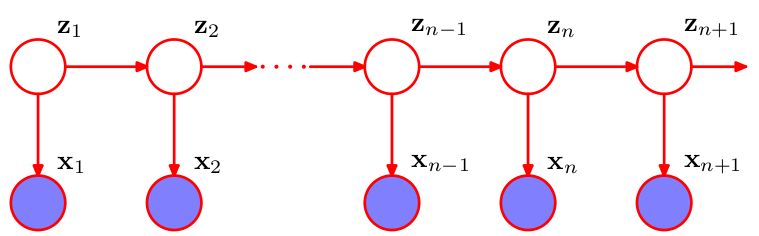
\includegraphics[scale=0.4]{hmm-chain.png}
  \end{center}
\end{frame}



\begin{frame}
  \frametitle{A real Markov process}
A dishonest casino
\hskip 2cm 
\includegraphics{dice.png}
\includegraphics{dice.png}
\includegraphics{dice.png}
  \begin{itemize}
  \item A casino has two dice:
    \begin{itemize}
    \item Fair die:     $P(1) = P(2) = P(3) = P(5) = P(6) = 1/6$
    \item Loaded die: \\
      $P(1) = P(2) = P(3) = P(5) = 1/10$\\
      $P(6) = 1/2$
    \end{itemize}
  \item Casino player switches back-and-forth between fair and loaded
    die once every 20 turns on average
  \end{itemize}
\end{frame}


 \begin{frame}
   \frametitle{\voc{Evaluation} question}
   \begin{itemize}
   \item Given a sequence of rolls:\\
     124552\alert{6}4\alert{6}214\alert{6}14\alert{6}13\alert{6}13\alert{6}\alert{6}\alert{6}1\alert{6}\alert{6}4\alert{6}
     \alert{6}1\alert{6}3\\\alert{6}\alert{6}1\alert{6}3\alert{6}\alert{6}1\alert{6}3\alert{6}1\alert{6}515\alert{6}1511514\alert{6}1235\alert{6}2344
  \item How likely is this sequence, given our model of the casino?
   \end{itemize}
 \end{frame}


 \begin{frame}
   \frametitle{\Large \voc{Decoding} question} 
   \begin{itemize}
   \item Given a sequence of rolls:\\
       124552\alert{6}4\alert{6}214\alert{6}14\alert{6}13\alert{6}13\alert{6}\alert{6}\alert{6}1\alert{6}\alert{6}4\alert{6}
       \alert{6}1\alert{6}3\\\alert{6}\alert{6}1\alert{6}3\alert{6}\alert{6}1\alert{6}3\alert{6}1\alert{6}515\alert{6}1511514\alert{6}1235\alert{6}2344
   \item Which throws were generated by the fair dice and which by the
     loaded dice?
   \end{itemize}
 \end{frame}


 \begin{frame}
   \frametitle{\voc{\large Learning} question}
   \begin{itemize}
   \item Given a sequence of rolls:\\
       124552\alert{6}4\alert{6}214\alert{6}14\alert{6}13\alert{6}13\alert{6}\alert{6}\alert{6}1\alert{6}\alert{6}4\alert{6}
       \alert{6}1\alert{6}3\\\alert{6}\alert{6}1\alert{6}3\alert{6}\alert{6}1\alert{6}3\alert{6}1\alert{6}515\alert{6}1511514\alert{6}1235\alert{6}2344
   \item Can we infer how the casino works? How loaded is the dice? How
     often the casino player changes between the dice?
\end{itemize}
 \end{frame}

 \begin{frame}
   \frametitle{The dishonest casino model}
   \begin{center}
     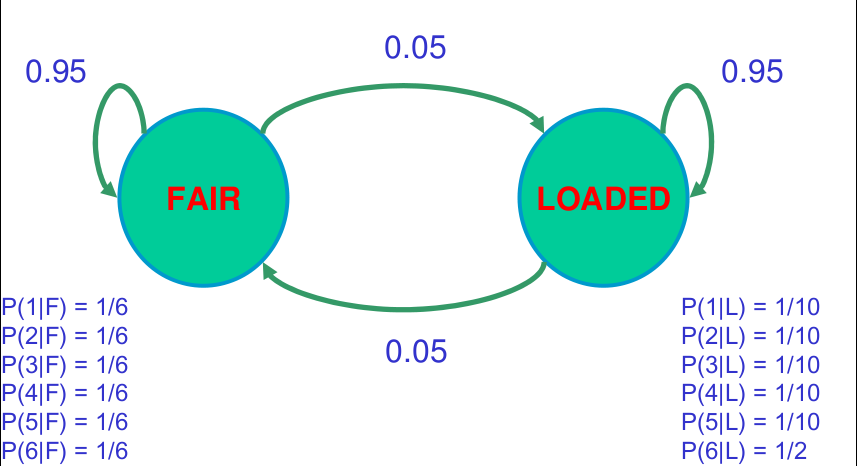
\includegraphics[scale=0.4]{dishonest-casino.png}
   \end{center}
 \end{frame}

 \begin{frame}
   \frametitle{Example}
\vskip -0.8cm
\hskip 9cm 
\includegraphics{dice.png}
\begin{itemize}
\item Let the sequence of rolls be:
  $\x = (1,2,1,5,2,1,6,2,4)$
\item A candidate \voc{parse} is $\z = (F,F,F,F,F,F,F,F,F,F)$
\item What is the probability $P(\x,\z)$?
  \begin{align*}
     P(\x,\z) = \prod_{i=1}^N P(x_i|z_{i})
                         P(z_i|z_{i-1})
  \end{align*}
\item (Let's assume initial transition probabilities $P(F|0) = P(L|0)
  = \frac{1}{2}$)
\pause
  \begin{align*}
    & \frac{1}{2} \times P(1|F)P(F|F) \times P(2|F) P(F|F) \cdots
    P(4|L)\\
\pause
    & = \frac{1}{2} \times \left(\frac{1}{6}\right)^{10} \times 0.95^9\\
    & = 5.21 \times 10^{-9}
  \end{align*}
\end{itemize}
 \end{frame}


 \begin{frame}
      \frametitle{Example}
\vskip -0.8cm
\hskip 9cm 
\includegraphics{dice.png}
\begin{itemize}
  \item What about the parse $\z = (L,L,L,L,L,L,L,L,L,L)$?
    \begin{align*}
      & \frac{1}{2} \times P(1|L)P(L|L) \times P(2|L) P(L|L) \cdots
      P(4|L)\\
      & = \frac{1}{2} \times 0.5^2 \times 0.95^0 = 7.9 \times 10^{-10}
    \end{align*}
  \item It's 6.61 times more likely that the all the throws came from
    a fair dice than that they came from a loaded dice.
\end{itemize}
 \end{frame}


 \begin{frame}
      \frametitle{Example}
\vskip -0.8cm
\hskip 9cm 
\includegraphics{dice.png}
\begin{itemize}
\item Now let the throws be: $\x = (1,6,6,5,6,2,6,6,3,6)$
\item What is $P(\x,F^{10})$ now?  
  \pause
  \begin{align*}
    \frac{1}{2} \times \left(\frac{1}{6}\right)^{10} \times 0.95^9 = 5.21 \times 10^{-9}
  \end{align*}
  \alert{Same as before}
  \pause
\item What is  $P(\x,L^{10})$
  \pause
  \begin{align*}
    \frac{1}{2} \times 0.1^4 \times 0.5^6 \times 0.95^9 = 0.5 \times 10^{-7}
  \end{align*}
\item So now it is 100 times more likely that all the throws came from
  a loaded dice
\end{itemize}
\end{frame}


\begin{frame}
  \frametitle{Decoding}
  \begin{itemize}
  \item Given $\x$ we want to find the best $\z$, i.e.\ the one which
    maximizes $P(\x,\z)$
    \[
    \hat{z} = \argmax_{\z} P(\x,\z)
    \]
  \item Enumerate all possible $\z$, and evalue $P(\x,\z)$?
    \pause
  \item Exponential in length of input
    \pause
  \item Dynamic programming to the rescue
  \end{itemize}
\end{frame}

\begin{frame}
  \frametitle{Decoding}
  \begin{center}
    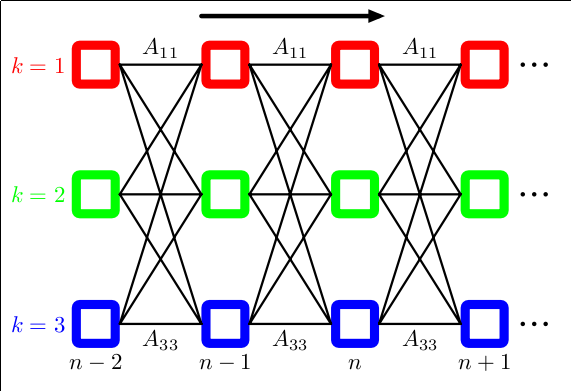
\includegraphics[scale=0.3]{grid.png}
  \end{center}

  \begin{itemize}
  \item Store intermediate results in a table for reuse
  \item Score to remember: probability of the most likely sequence of
    states up to position $i$, with state at position $i$ being $k$
    \begin{block}{}
      \begin{align*}
        V_k(i) = \max_{z_1,\ldots,z_{i-1}}
        P(x_1,\cdots,x_{i-1},z_1,\cdots,z_{i-1},x_i,z_i=k)
      \end{align*}

    \end{block}
  \end{itemize}
\end{frame}


\begin{frame}
  \frametitle{Decoding}
  \begin{itemize}
  \item We can define $V_k(i)$ recursively
    \begin{align*}
      V_l(i+1) & = \max_{z_1,\ldots,z_i}
      P(x_1,\ldots,x_i,z_1,\ldots,z_i,x_{i+1},z_{i+1} = l)\\
      & = \max_{z_1,\ldots,z_i}
      P(x_{i+1},z_{i+1}=l|x_1,\ldots,x_i,z_1,\ldots,z_i)\\
      & ~~~~~~~~ \times P(x_1,\ldots,x_i,z_1,\ldots,z_i)\\
      & = \max_{z_1,\ldots,z_i}
        P(x_{i+1},z_{i+1}=l|z_i)P(x_1,\ldots,x_i,z_1,\ldots,z_i)\\
      & = \max_k P(x_{i+1},z_{i+1} = l) \max_{  z_1,\ldots,z_{i-1}}
      P(x_1,\cdots,x_{i},z_1,\cdots,z_i=k)\\
      & = \max_k P(x_{i+1},z_{i+1} = l) V_k(i)\\
      & = P(x_{i+1}|z_{i+1} = l) \max_k P(z_{i+1}=k|z_{i}=l) V_k(i)
    \end{align*}
\item We introduce simplified notation for the parameters
  \begin{block}{}
    \begin{align*}
      V_l(i+1) = E_l(x_{i+1}) \max_k A_{kl} V_k(i)
    \end{align*}
  \end{block}
  \end{itemize}
\end{frame}

\begin{frame}
  \frametitle{Viterbi algorithm}
  \begin{block}
    {}
    \begin{itemize}
    \item Input $\x = (x_1,\ldots,x_N)$
    \item Initialization
      \begin{align*}
        V_0(0) = 1 & \text{ where 0 is the fake starting position}\\
        V_k(0) = 0 & \text{ for all } k > 0
      \end{align*}
    \item Recursion
      \begin{align*}
        V_l(i) & = E_l(x_{i}) \max_k A_{kl} V_k(i-1)\\
        Z_l(i) & = \argmax_k A_{kl} V_k(i-1)
      \end{align*}
    \item Termination
      \begin{align*}
        P(\x,\hat{\z}) & = \max_k V_k(N)\\
        \hat{z_N} & = \argmax_k V_k(N)
      \end{align*}
    \item  Traceback
      \begin{align*}
        \hat{z}_{i-1} & = Z_{z_i}(i)
      \end{align*}
    \end{itemize}
  \end{block}
\end{frame}


\begin{frame}
  \frametitle{Learning HMM}
  \begin{itemize}
  \item Learning from labeled data
    \pause
    \begin{itemize}
    \item Estimate parameters (emission and transition probabilities)
      from (smoothed) relative counts
      \pause
      \begin{align*}
        A_{kl} & = \frac{C(k,l)}{\sum_{l'} C(k,l')}
      \end{align*}
      \begin{align*}
        E_k(x) & = \frac{C(k,x)}{\sum_{x'} C(k,x')}
      \end{align*}
    \end{itemize}
  \item Learning from unlabeled with Expectation Maximization
      \begin{itemize}
      \item Start with randomly initialized parameters $\theta_0$
      \item Iterate until convergence
        \begin{itemize}
        \item Compute (soft) labeling given current $\theta_i$
        \item Compute updated parameters $\theta_{i+1}$ from this labeling
        \end{itemize}
      \end{itemize}
  \end{itemize}
\end{frame}

\section{Maximum Entropy Markov Models}
\begin{frame}
  \frametitle{Maximum Entropy Markov Models}
  \begin{itemize}
  \item Model structure like in HMM
  \item Logistic regression (Maxent) to learn $P(z_i|\x,z_{i-1})$
  \item For decoding, use learned probabilities and run Viterbi
  \end{itemize}
\end{frame}

\begin{frame}
  \frametitle{HMMs and MEMMs}
  \begin{itemize}
  \item HMM POS tagging model:
    \begin{align*}
      \hat{\z} & = \argmax_\z P(\z|\x) \\
      & = \argmax_\z P(\x|\z)P(\z)\\
      & = \argmax_\z \prod_i P(x_i|z_i) P(z_i|z_{i-1})
\end{align*}
\item MEMM POS tagging model:
\begin{align*}
 \hat{\z} & = \argmax_\z P(\z|\x) \\
	 & = \argmax_\z \prod_i \alert{P(z_i|\x,z_{i-1})}
\end{align*}
\item Maximum entropy model gives conditional probabilities
\end{itemize}
\end{frame}

\begin{frame}\frametitle{Conditioning probabilities in a HMM and a
    MEMM}
 \begin{center}
 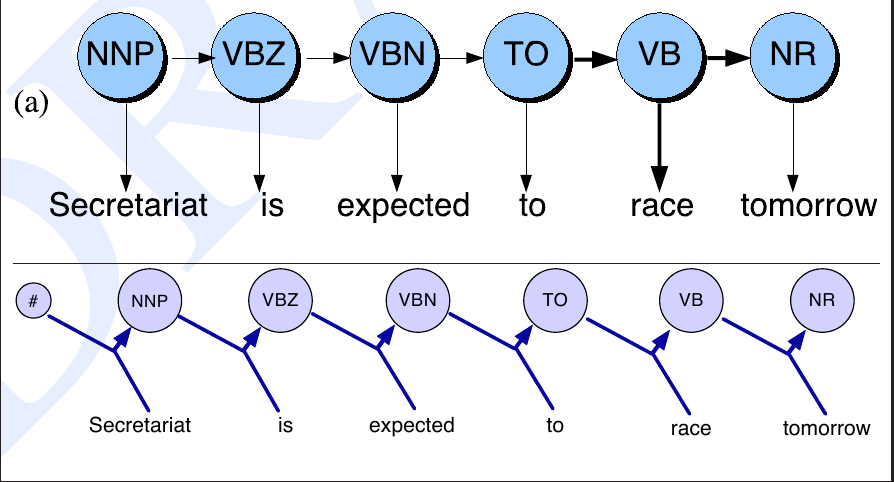
\includegraphics[scale=0.3]{hmm-memm.png}
 % hmm-memm.png: 894x482 pixel, 72dpi, 31.54x17.00 cm, bb=0 0 894 482
\end{center}
\end{frame}


\begin{frame}
 \frametitle{Viterbi in MEMMs}
 \begin{itemize}
 \item Decoding works almost the same as in HMM
 \item Except entries in the DP table are values of
   $P(z_i|\x,z_{i-1})$
 \item Recursive step: Viterbi value of time $t$ for state $j$:
   \begin{equation*}
     V_l(i+1) = \max_k P(z_{i+1}=l|\x,z_i = k) V_k(i)
   \end{equation*}
 \end{itemize}
\end{frame}


% \begin{frame}
%  \frametitle{MaxEnt with beam search}
% \begin{equation}
%  P(z_1,...,z_n|x_1,...,x_n) = \prod_{i=1}^n P(z_i|x_i)
% \label{maxent-tagging-eq}
% \end{equation}

% \begin{block}{Beam search}
%   The beam search algorithm maintains the $N$ highest scoring tag
%   sequences up to the previous word.

%   \vskip 0.5cm Each of those label sequences is combined with the
%   current word $x_i$ to create the context $c_i$, and the Maximum
%   Entropy Model is used to obtain the $N$ probability distributions
%   over tags for word $w_i$.

%   \vskip 0.5cm Now we find $N$ most likely sequences of tags up to and
%   including word $w_i$ by using Equation \ref{maxent-tagging-eq}, and
%   we proceed to word $w_{i+1}$.
% \end{block}
% \end{frame}




\section{Sequence perceptron}

\begin{frame}
  \frametitle{Perceptron for sequences}
%Described in \cite{1118694}

\begin{block}{\textsc{SequencePerceptron}($\{\x\}^{1:N},\{\z\}^{1:N},I$):}
\begin{algorithmic}[1]
\STATE $\w \leftarrow \vecb{0}$
\FOR {$i = 1...I$}
	\FOR {$n = 1...N$}
		\STATE $\hat{\y}^{(n)} \leftarrow \argmax_\z \w \cdot \Phi(\x^{(n)},\z)$ \label{argmax-line}
    		\IF {$\hat{\z}^{(n)} \neq \z^{(n)}$}
        		\STATE $\w \leftarrow \w + \Phi(\x^{(n)},\z^{(n)}) - \Phi(\x^{(n)},\hat{\z}^{(n)})$

    		\ENDIF
    	\ENDFOR
\ENDFOR
\STATE \textbf{return} $\w$
\end{algorithmic}                 
\end{block}
\end{frame}



\begin{frame}\frametitle{Feature function}



  \begin{center}
    \alert{Harry}$_{\text{PER}}$ loves$_\text{O}$
    \alert{Mary}$_{\text{PER}}$
  \end{center}


\[
\Phi(\x,\z) = \sum_i \phi(\x,z_{i-1},z_i)
\]


\begin{footnotesize}
  \begin{tabular}{l|ccc}
    $i$ 
               & $x_i=\text{Harry}\wedge z_i=\text{PER}$
               & $\mathrm{suff}_2(x_{i})=\text{ry} \wedge z_i=\text{PER}$
               & $x_i=\text{loves}\wedge z_i=\text{O}$ \\
   1           & 1 & 1 & 0 \\
   2           & 0 & 0 & 1 \\
   3           & 0 & 1 & 0 \\\hline
  $\Phi$       & 1 & 2 & 1 \\
  \end{tabular}  
\end{footnotesize}
\end{frame}


\begin{frame}
  \frametitle{Search}
\begin{block}{}
\[
\hat{\z}^{(n)} = \argmax_\z \w \cdot \Phi(\x^{(n)},\z)
\]
\end{block}
Global score is computed incrementally:

\[
\w \cdot \Phi(\x,\z) = \sum_{i=1}^{|\x|}\w~\cdot~\phi(\x,z_{i-1},z_i)
\]
\end{frame}


\begin{frame}
  \frametitle{Update term}
\begin{block}{}
\[
\w^{(n)} = \w^{(n-1)} + \left[ \Phi(\x^{(n)},\z^{(n)}) - \Phi(\x^{(n)},\hat{\z}^{(n)})
\right]
\]
\end{block}

\[
\begin{aligned}
&    &&  \Phi(\text{\small Harry loves Mary},\text{\small PER O PER}) \\
& -  &&  \Phi(\text{\small Harry loves Mary},\text{\small ORG O PER}) = 
\end{aligned}
\]

\begin{scriptsize}
  \begin{tabular}{cccc}
                 $x_i=\text{Harry}\wedge z_i=\text{PER}$
               & $x_i=\text{Harry}\wedge z_i=\text{ORG}$
               & $\mathrm{suff}_2(x_{i})=\text{ry} \wedge z_i=\text{PER}$
               & $\cdots$ \\\hline
 1 & 0  & 2 & $\cdots$ \\
 0 & 1  & 1 & $\cdots$ \\\hline
 1 & -1 & 1 & $\cdots$ \\
\end{tabular}
  
\end{scriptsize}
\end{frame}


\begin{frame}
  \frametitle{Comparison}
  \begin{center}
    \begin{tabular}{l|lll}
      Model         & HMM           & MEMM             & Perceptron \\\hline
      Type          & Generative    & Discriminative   & Discriminative \\
      Distribution  & $P(\x,\z)$    & $P(\z|\x)$       & N/A\\
      Smoothing     & Crucial       & Optional         & Optional \\
      Output   dep. & Chain         & Chain            & Chain \\
      Sup. learning & No decoding   & No decoding      & With decoding \\
    \end{tabular}
  \end{center}

\end{frame}

\begin{frame}
  \frametitle{The end}
\end{frame}
\end{document}
